\documentclass[11pt,a4paper]{jsarticle}

\usepackage[dvipdfmx]{graphicx}
\usepackage{graphicx}
\usepackage[top=20truemm,bottom=20truemm,left=25truemm,right=25truemm]{geometry}
\usepackage{comment}
%\usepackage[style=phys,articletitle=false,biblabel=brackets,chaptertitle=false,pageranges=false]{biblatex}

%https://qiita.com/Toru3/items/7ea1342da1e31f0c28c3
\usepackage{fancyhdr}
\usepackage{lastpage}
\fancypagestyle{mypagestyle}{%
\lhead{\thepage/\pageref{LastPage}}%ヘッダ左
\rhead{留学先での研究テーマ 平松信義}%ヘッダ右
\cfoot{}%\thepage/\pageref{LastPage}}%フッタ中央に"今のページ数/総ページ数"を設定
\renewcommand{\headrulewidth}{0.0pt}%ヘッダの線を消す
}
\pagestyle{mypagestyle}

\title{留学先での研究テーマ\\準粒子からなるボース・アインシュタイン凝縮体の光制御と応用}
\author{東京大学工学部物理工学科 平松信義}
\date{\today}

\begin{document}
\maketitle
\thispagestyle{mypagestyle}

\section{背景}
\subsection{光技術を用いたボース・アインシュタイン凝縮の観測}
ボース・アインシュタイン凝縮(BEC)は、低温で近接するボース粒子同士が量子力学的な干渉をして、最低エネルギー状態に落ち込む現象である。ボース凝縮体において粒子はお互いに協調してふるまい、巨視的な量子効果があらわになる。
ボース粒子がお互いに干渉してBECが観測できるための条件は、ボース粒子の波束の広がりがボース粒子間の平均的な距離に対して長いことである。ボース粒子の波束の広がりは、以下の熱的ド・ブロイ長$\lambda_{\rm TdB}$で特徴づけられる。
\begin{eqnarray}
\lambda_{\rm TdB} &=& \frac{h}{\sqrt{2\pi m^* k_B T}}.
\label{eq:lambda}
\end{eqnarray}
ただし$h$はプランク定数、$k_B$はボルツマン定数、$m^*$はボース粒子の有効質量である。温度を低くすれば熱的ド・ブロイ長$\lambda_{\rm TdB}$は大きくなり、ある温度以下でBECの観測が可能になる。%また実現できる温度に下限が存在しても、十分にボース粒子の有効質量が小さくまた十分に粒子が密に存在していれば、その系でBECの観測は可能になる。

アインシュタインの1925年の予言以来、BECは明らかな形で確認されていなかったが、1995年に低温の希薄ガス中で観測された
\cite{Davis,Anderson}。磁気光学トラップ(MOT)と呼ばれるレーザー光を用いた粒子閉じ込め方法と、蒸発冷却と呼ばれる冷却手法のブレークスルーが、BECの実現につながった。%それ以来MOTと蒸発冷却は希薄ガスのBECを実現する標準的な方法となった。
MOTは非一様磁場中に偏光した光を入射する手法で、粒子は空間的に束縛されボース粒子の密度は大きくなる。そのあと様々な物質の系でBECは実現されているが、光を用いた冷却とトラップ技術はその多くで用いられ\cite{ketterle}、BECを実現するために極めて有用である。

またBECに関して現在知られているほぼ全てのことは光を用いた探査法によって得られたたものである\cite{ketterle}。光学測定には接触方式と異なり、系への熱の流入を防げるという大きな利点がある。またボース粒子の時間依存する分布を非破壊に見たり、吸収・散乱からエネルギースペクトルなどを測定できるといった測定の多様さも有利である。実際、希薄ガスのBECの検出には光学系が広く用いられており、後述する励起子\cite{Lin,Yoshioka}やフォノン\cite{Misochko}のBEC状態に関する実験でも励起と計測に光技術が用いられている。

\subsection{励起子のBEC}
励起子は結晶をバンド理論で記述した時に現れる電子と正孔がクーロン引力により束縛状態を作ったものである。
また励起子は準粒子と呼ばれるエネルギー量子の一つであり、結晶中に現れるボース粒子と捉えられる。
励起子のBECはこれまで理論的に予測されていたが\cite{Blatt}、励起子同士の相互作用から有限の寿命を持っており、ボース・アインシュタイン凝縮体が実際に形成されるかどうかは自明でなかった。

励起子のBECを検出するために近年まで酸化銅${\rm Cu_2O}$を中心に着実な実験研究が進められてきた\cite{Lin,David}。しかし励起子は相互作用するため、多くの物質でBECを実現するには温度数K 以下の超低温が必要であり、実証的な実験は困難だった。しかし近年温度数百mKでBECに伴う緩和爆発が検出された\cite{Yoshioka}。これは励起子のBECを直接示した実験証拠と考えられている。

\section{留学先での研究テーマ}
\subsection{励起子のBEC波動関数の干渉}
第一のテーマでは励起子のBEC状態を二つ用意し、それらの巨視的な波動関数の干渉を示すことを目標とする。この干渉はすでに希薄ガスのBEC状態で観測されているが\cite{Shin}、筆者の知る限り励起子に関してはまだ観測されていない。この干渉の観測は物質の巨視的な波動関数の制御につながる重要なステップである。
文献\cite{Lin,Yoshioka}において、レーザーパルスにより励起された励起子はCu$_2$O結晶の歪みにトラップされBECを起こした。歪みによるトラップをMOTまたは他の光学トラップに置き換えることができるなら、希薄ガスで実現されているような巨視的なBEC波動関数の干渉を結晶中でも観測できると筆者は考える。

\subsection{励起子のBEC状態を用いた半導体レーザーの評価・実証研究}
第二のテーマでは励起子のBEC状態を活用した半導体レーザーを評価し、その動作を実証することを目標とする。
通常の半導体レーザーは励起子を形成する電子と正孔が結合する際に誘導放射現象を起こすことで発光する。
BEC状態にある励起子は非常にコヒーレンスの高い状態である。近年BEC状態にある励起子が誘導放射により発光すると周波数にサブバンドが現れることが示された\cite{Horikiri}。この結果は新しい原理によるレーザーの開発につながるものであるが、いまだ発光の詳しいメカニズムは明らかにされていない。

\subsection{結晶中の準粒子のBECの観測}
第三のテーマは、励起子以外の準粒子がなすBEC状態を観測することを目標とする。
励起子の多体系でBECを観測できたことは、今後結晶中の他の準粒子に関してBECが実現できる可能性を示唆する。例えばすでにフォノンに関してはBEC状態が報告されている\cite{Misochko}。
励起子のBECを観測した実験で励起子の質量は小さく、式\ref{eq:lambda}から熱的ド・ブロイ長$\lambda_{\rm TdB}$は大きい。このように小さな質量を持つ他の準粒子でもBECを実現できると、比較的高温でBECが観測でき、結晶中の多様な量子効果の実証研究に有用である。超伝導体中に現れるボゴリューゴフ粒子にBECが起きているかどうかは論争の的である。実験で確認できれば極めて有益な結果になると考える。

%研究室
\section{希望する研究室}
筆者は中国の清華大学のMing-Fong Tai教授、Yi-Hsien Lee教授とHui Zhai教授の研究室を希望する。
Ming-Fong Tai教授は物理系学科に所属しており、新規超伝導材料の光学的な評価を行なっている\cite{Chang2}。
Yi-Hsien教授は物質工学系学科に所属しており、二次元物質に現れる励起子に関して実験研究を行なっている\cite{Mahmood}。
Hui Zhai教授は物理系学科に所属しており、非従来型のBEC現象に関する理論研究を行なっている\cite{Wang}。
%李信義(Yi-Hsien Lee), \UTF{7FDF}\UTF{835F}(Hui Zhai)

\section{筆者のこれまでの経験と留学先での研究}
筆者はこれまで光技術を用いた準粒子の特性評価に関わってきた。
筆者は表面プラズモンポラリトンの特性を体系的に評価し\footnote{研究論文の要旨1 (出版論文の要旨)}、アメリカ物理学協会(AIP)の雑誌に論文を出版した\cite{Hiramatsu}。表面プラズモンポラリトンは金属表面に現れる準粒子である。
アメリカのRice大学で行なった研究では、InSeに現れる励起子の偏光分解分光を行なった\footnote{ 図\ref{fig:poster}: Rice大学で研究発表した際に用いたポスター(参考)}。

また光計測実験の経験も持つ。東京大学の卒業研究ではIrTe$_2$の光誘起超伝導相の偏光顕微鏡を用いた分析に関わってきた\footnote{研究論文の要旨2 (卒業研究中間報告書の要旨)}。さらに半導体技術を用いた光計測技術に関してオーストリアの企業で開発研究に関わり、ヨーロッパ特許を出版した\cite{Etschmaier}。

以上の経験から本資料に記述した光技術とBECに関するテーマについて、留学先で比較的スムーズかつ効果的な研究を進めていけると筆者は自負している。

%\nocite{*}
\bibliography{SOP.bib}
\bibliographystyle{junsrt}

\begin{figure}[p]
  \begin{center}
   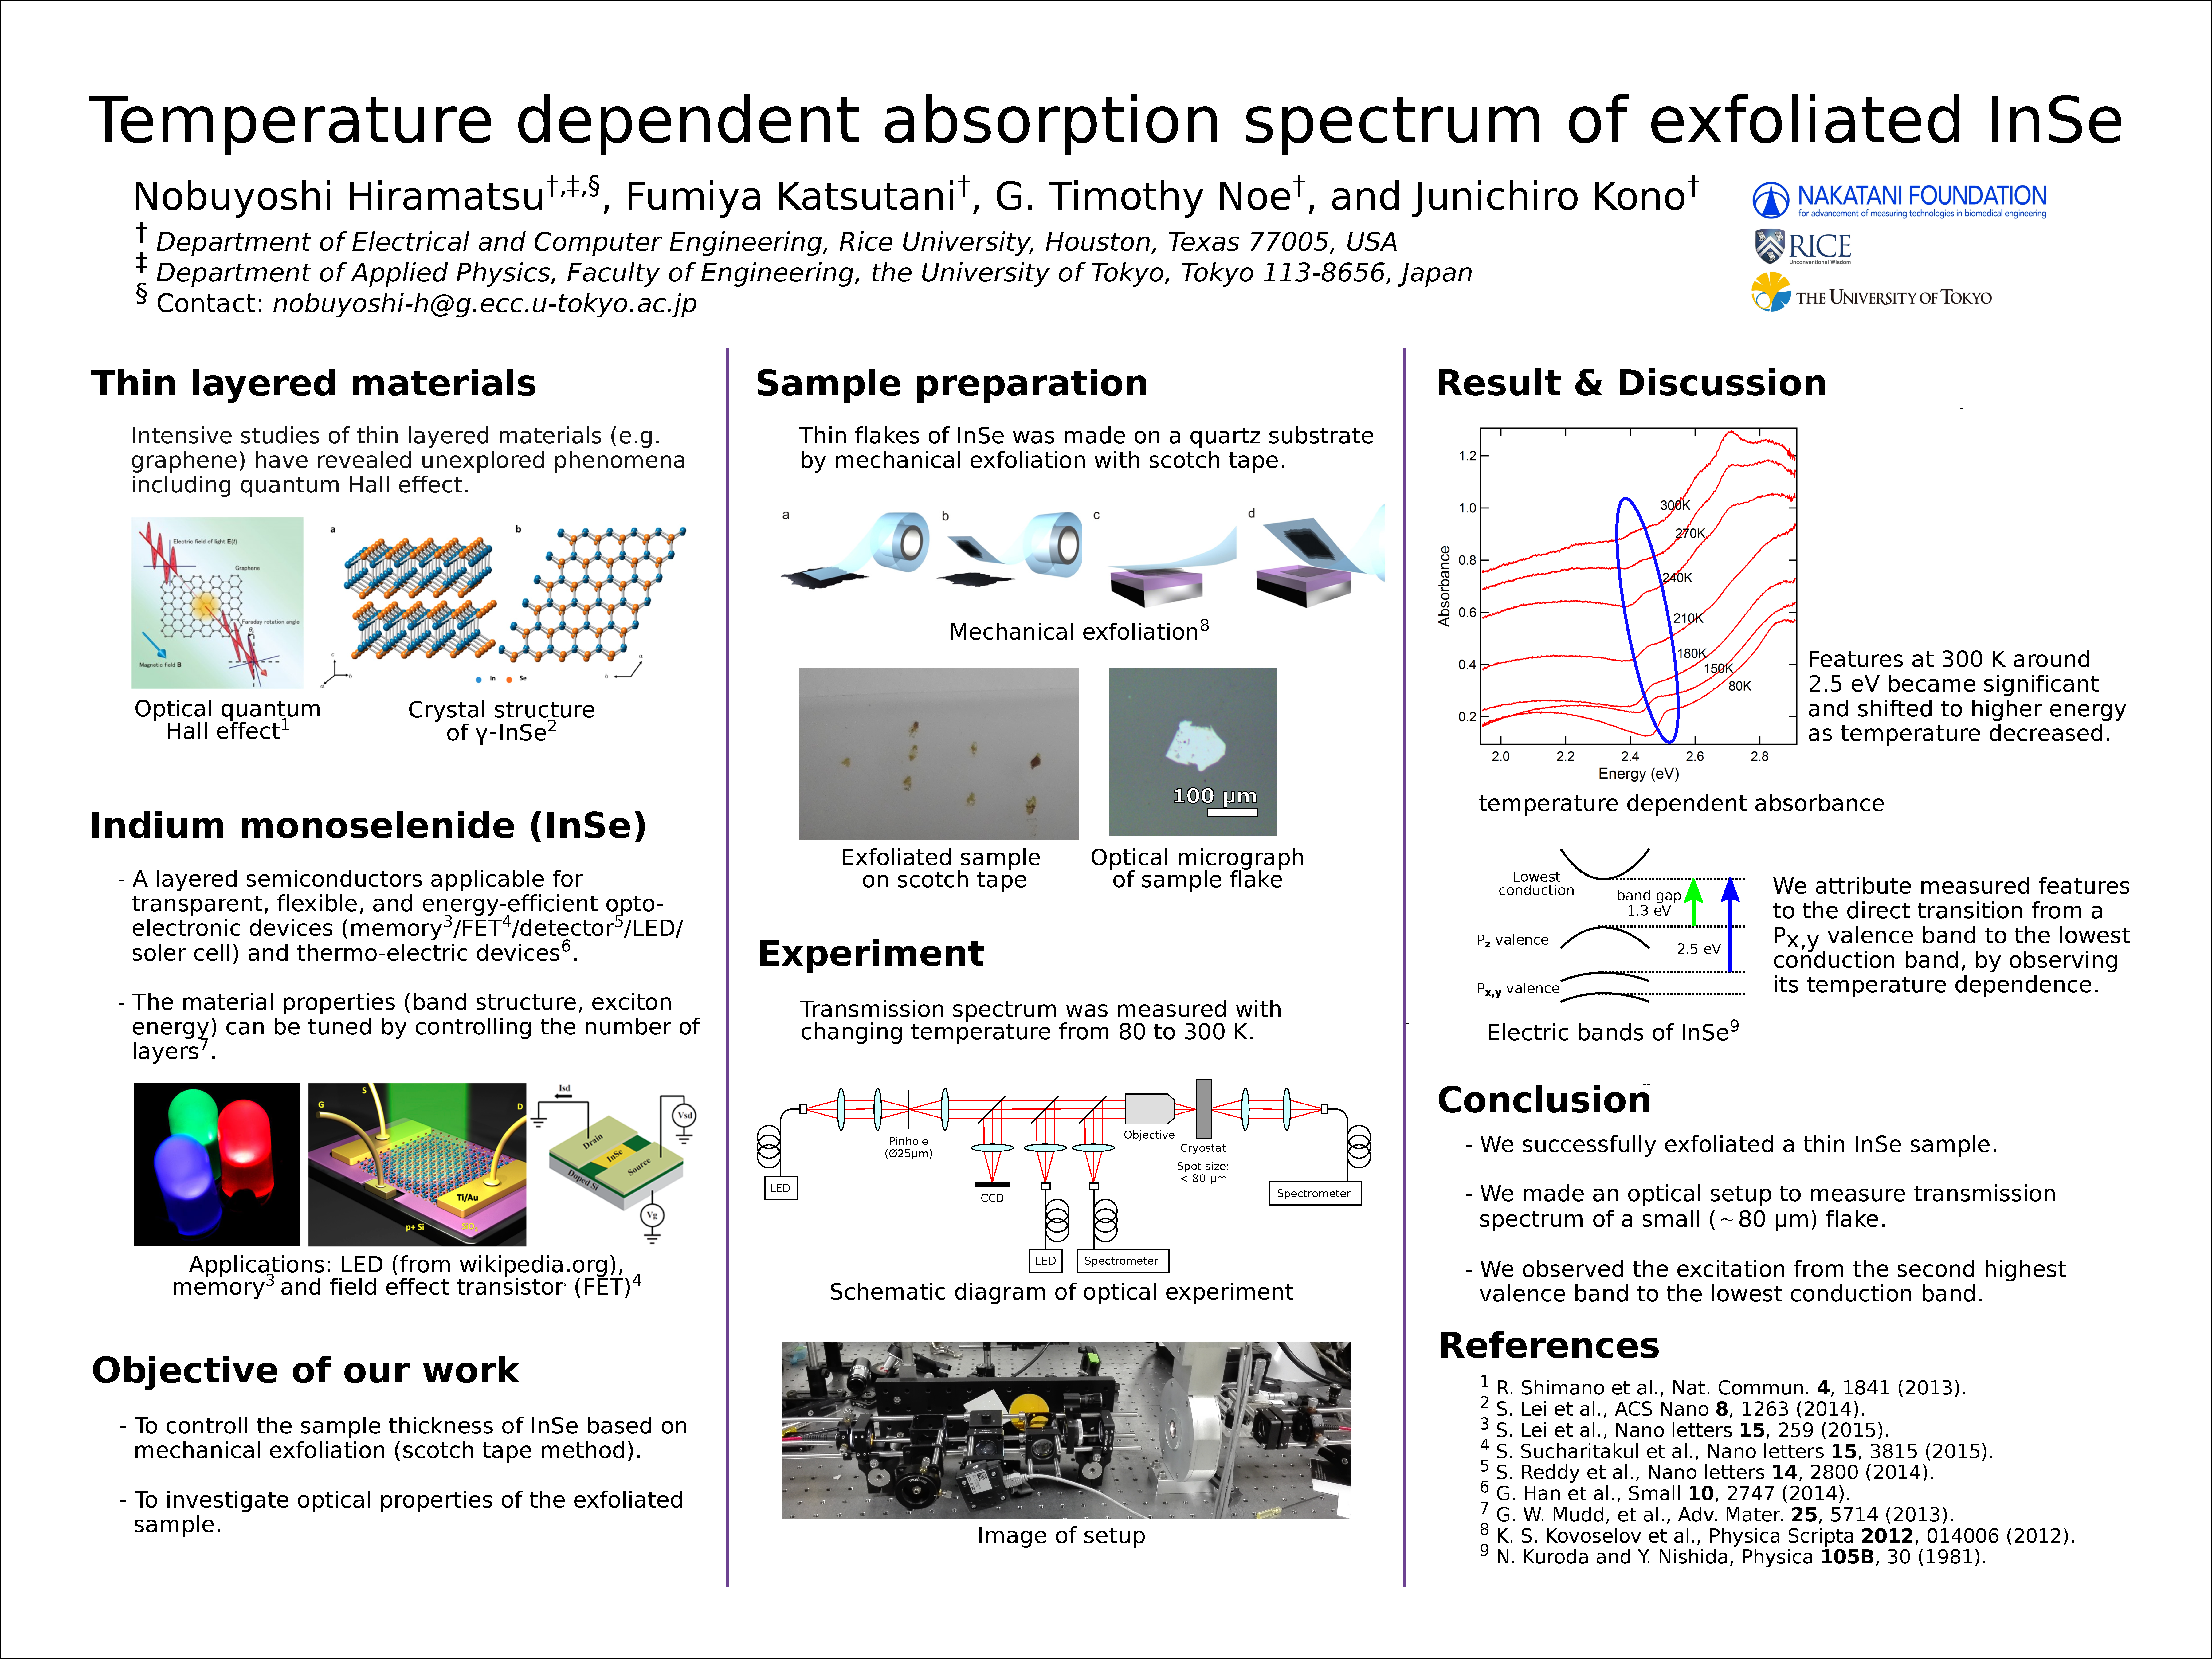
\includegraphics[width=1.4\hsize, angle=90]{poster_submitted.pdf}
  \end{center}
  \caption{Rice大学で研究発表した際に用いたポスター(参考)}
  \label{fig:poster}
\end{figure}


\end{document}
%コンパイルの仕方
%1. texファイルを一回コンパイル
%2. bibファイルを一回コンパイル
%3. texファイルを三回コンパイル